%%
%% Author: dariochinelli
%% 2021-03-15
%%
\section{Fenomeni spiegabili solo con l'esistenza dei fotoni}

\subsection{Produzione raggi X}

La produzione di raggi X è un fenomeno di interazione tra radiazione e materia, è una prova della doppia natura delle onde elettromagnetiche.
I raggi X di questo tipo vengono prodotti da un \underline{tubo a raggi X} in cui ho un fascio di elettroni accelerati mediante una differenza di potenziale di migliaia di Volt (ordine $10^5$V), precedentemente liberati per \textit{effetto termoionico} da un filamento di Tungsteno riscaldato.
Gli elettroni incidono sull'anodo che li ferma con una decelerazione molto repentina che porta all'emissione di uno spettro continuo di radiazione elettromagnetica.

\begin{figure}[h]
\centering
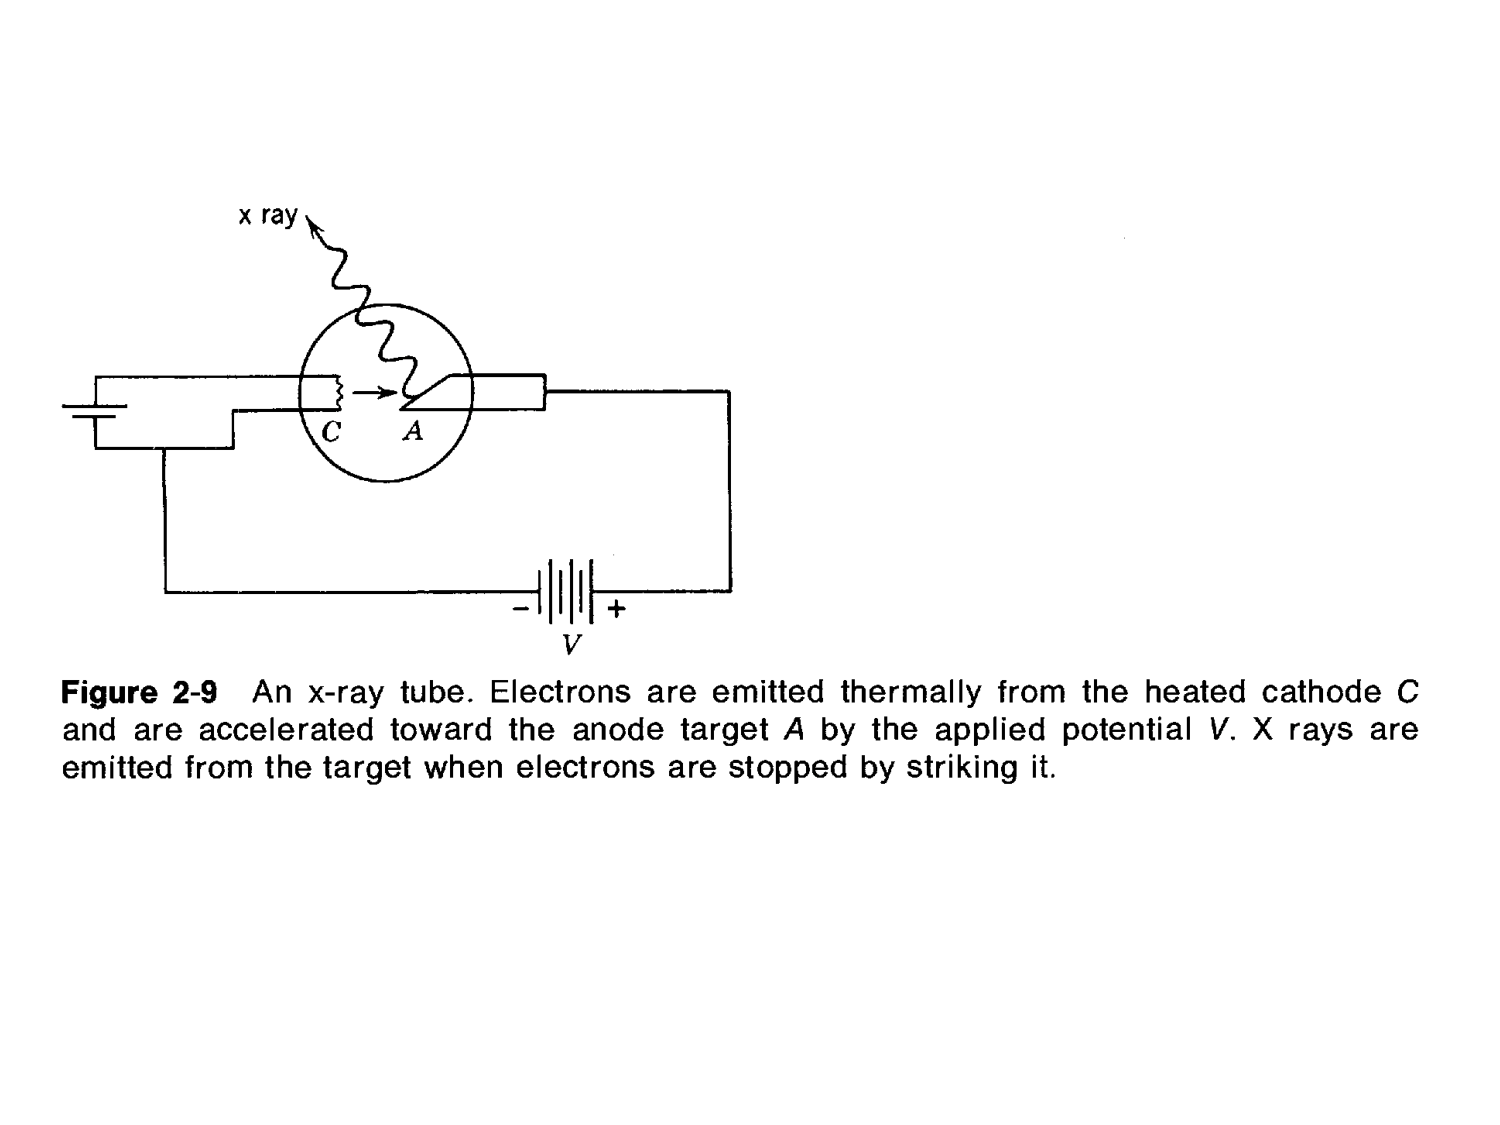
\includegraphics[scale=0.5]{/tubo_raggi_X}
\caption{Schema tecnico di produzione di raggi X}
\end{figure}

La $\lambda$ minima di emissione dipende solamente dall'energia applicata e non dal materiale di cui è costituito l'anodo.
\begin{figure}[h]
\centering
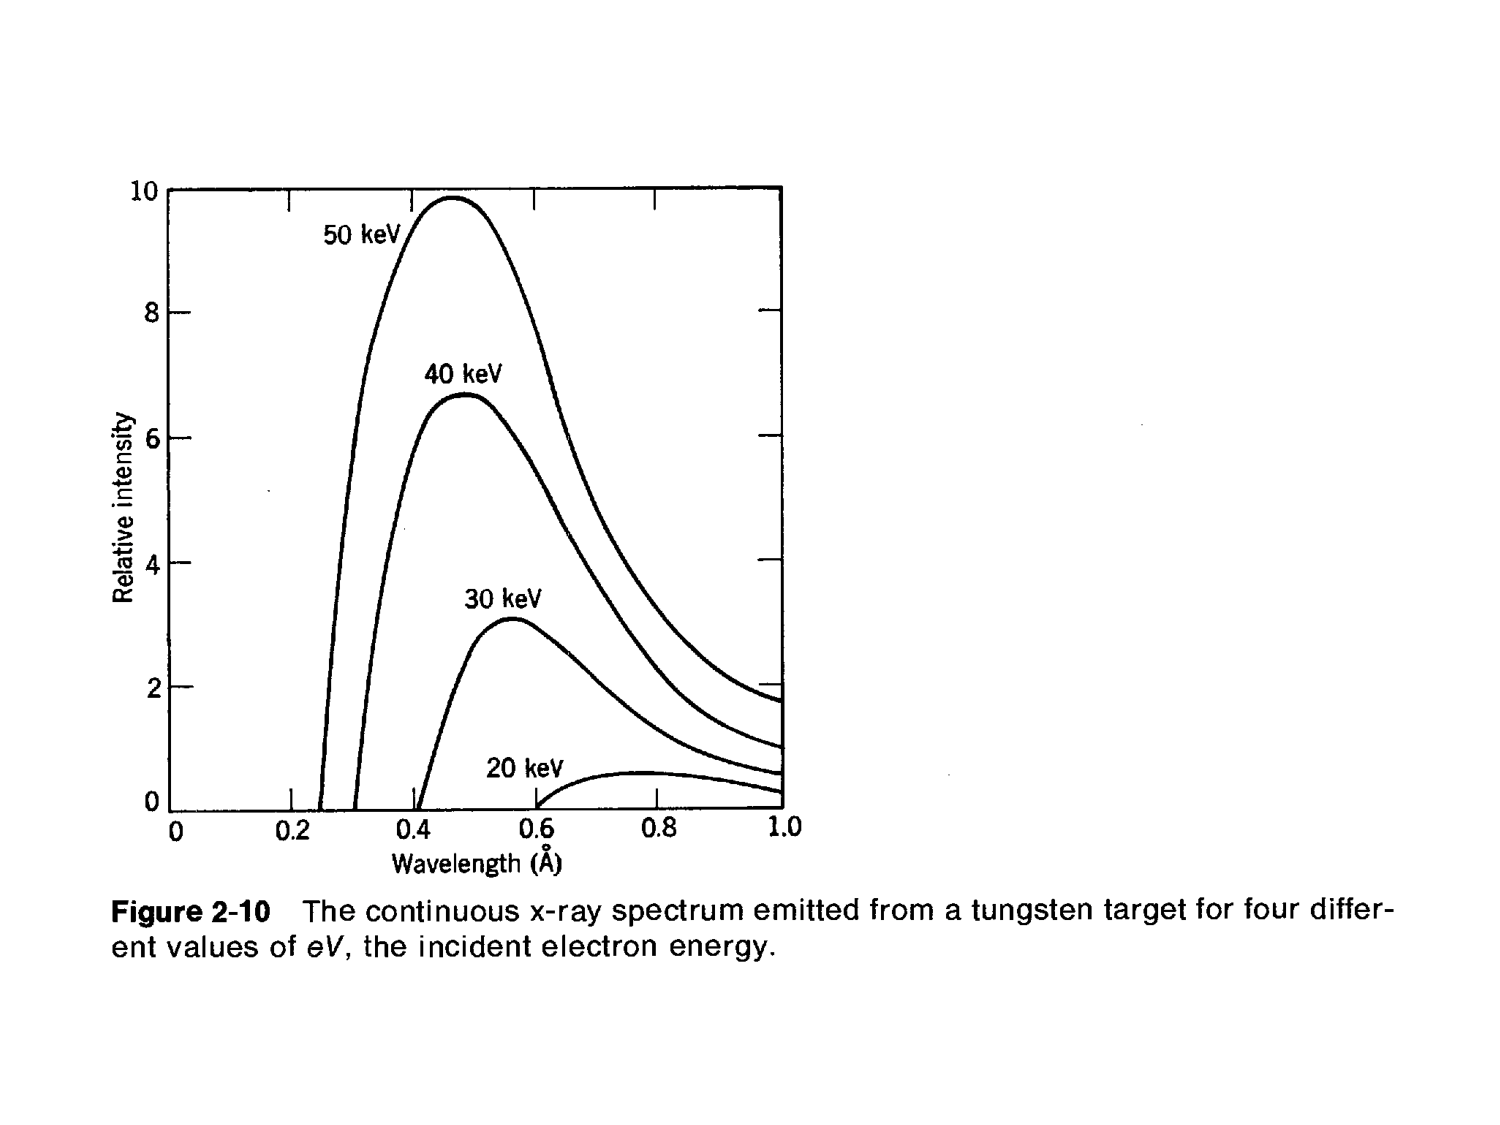
\includegraphics[scale=0.5]{/emissione_produzione_X}
\caption{Emissione che dipende solo dall'energia applicata nella differenza di potenziale}
\end{figure}

Questo fenomeno si spiega solo interpretando l'emissione come fotoni, fotoni X.
Un elettrone si fermerà dopo diverse interazioni di questo tipo, con una produzione continua di fotoni con diverse lunghezze d'onda,
variabile tra una $\lambda_{min}$ e infinito.
\begin{figure}[h]
\centering
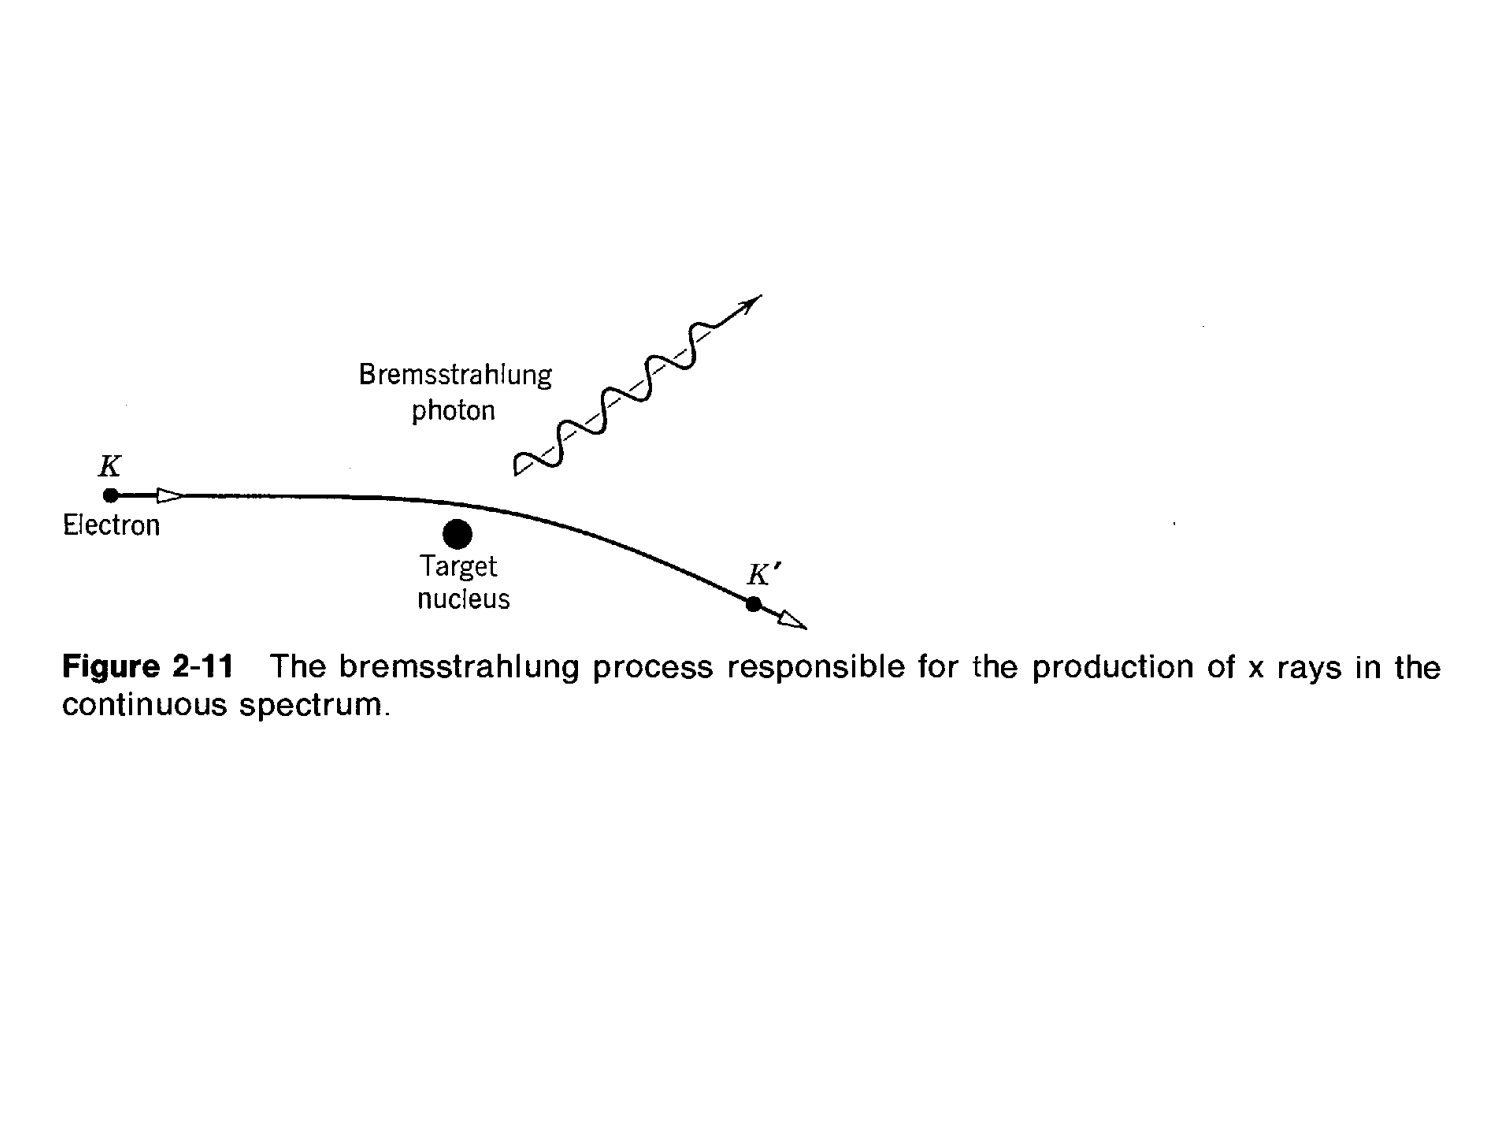
\includegraphics[scale=0.5]{/bremsstrahlung}
\caption{Schema interazione radiazione materia}
\end{figure}

\begin{equation}
\begin{split}
& h\nu = K - K' \\
& h \frac{ c}{\lambda } = K - K'
\end{split}
\end{equation}
Quando un elettrone perde tutta l'energia dopo un singolo evento ottengo la $\lambda$ minima:
\begin{equation}
\begin{split}
K' = 0 \quad & \Rightarrow \quad K = \frac{ hc}{\lambda_{min} } \\
eV = \frac{ hc}{\lambda_{min} } \quad & \Rightarrow \quad \lambda_{min} = \frac{ hc}{eV }
\end{split}
\end{equation}

Osservo che se la costante di Planck fosse nulla, la $\lambda_{min}$ tenderebbe a zero, ma così non è.
Questa radiazione elettromagnetica X è detta \textit{radiazione X di Bremsstrahlung}.

Si può vedere come l'inverso dell'effetto fotoelettrico!


\subsection{Produzione di coppie}

La produzione di coppie si verifica quando un fotone perde energia nell'interazione con un nucleo e si forma una coppia formata da un elettrone di energia $K_-$ e un positrone (particella analoga all'elettrone con carica positiva) di energia $K_+$.

\begin{figure}[h]
\centering
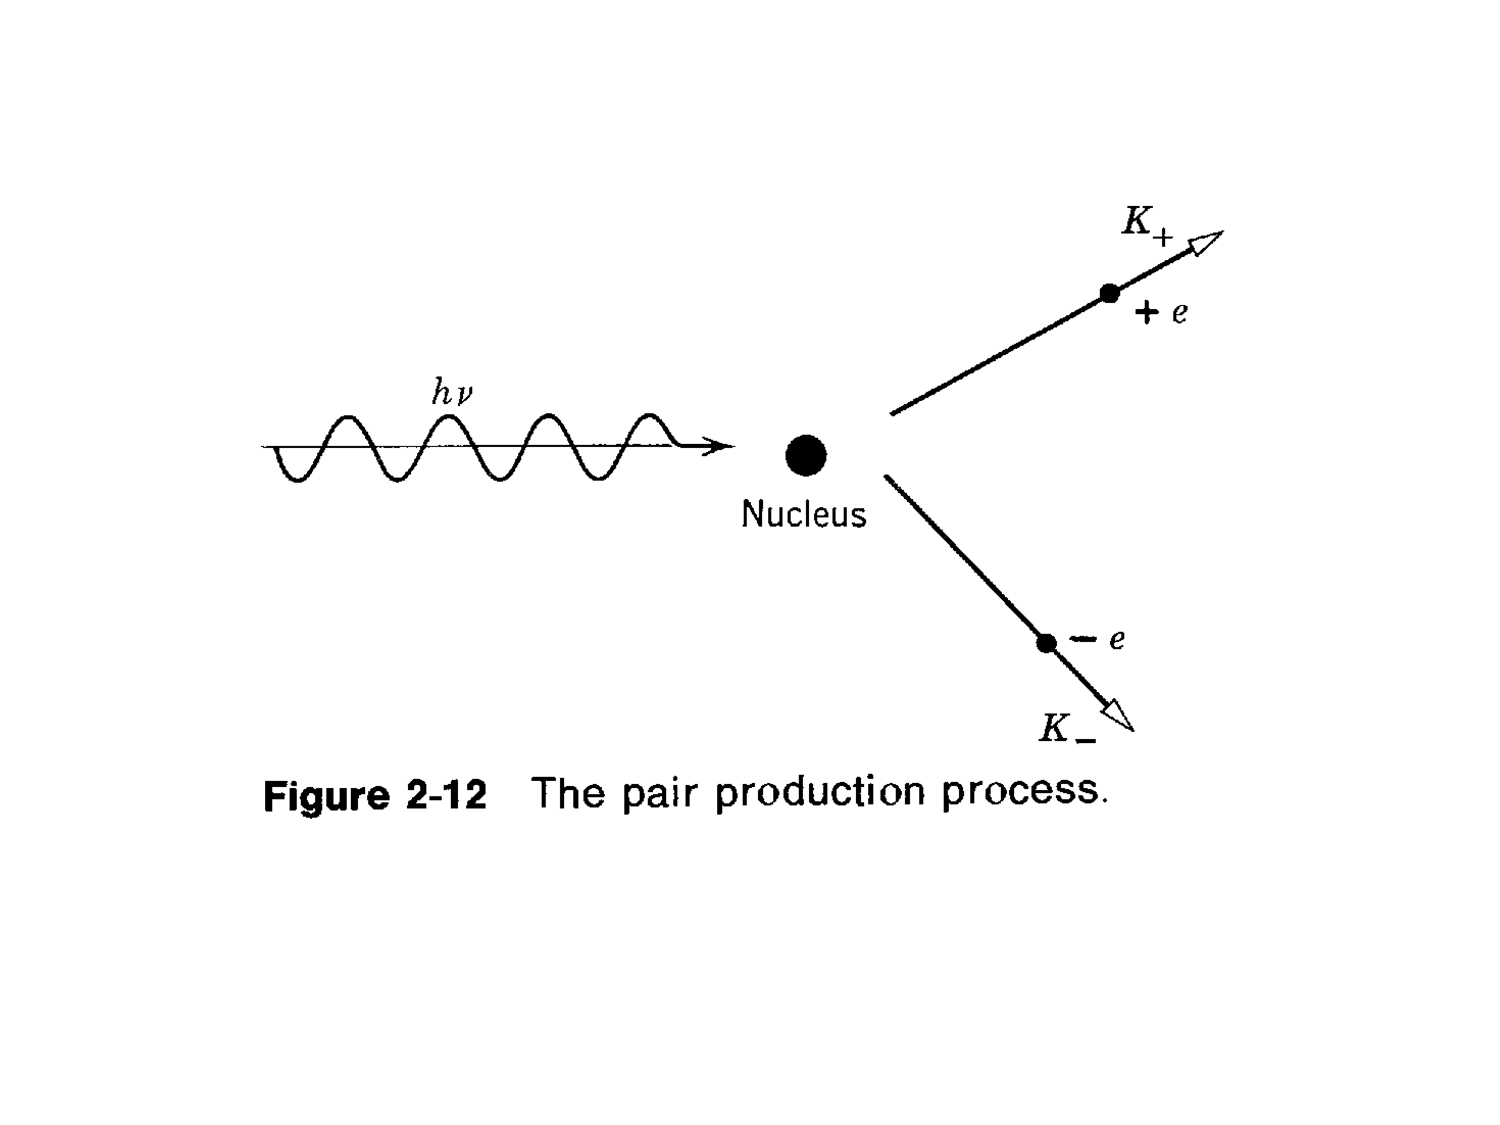
\includegraphics[scale=0.5]{/schema_pairproduction}
\caption{CAPTION}
\end{figure}

Eguagliando l'energia del fotone con la somma delle energie relativistiche delle due particelle si ottiene la cosiddetta \textit{energia di soglia}, ovvero l'energia minima del fotone per creare la coppia.

\begin{equation}
\begin{split}
& h\nu = E_- + E_+ = (m_0 c^2 + K_-) + (m_0 c^2 + K_+) = K_- + K_+ + 2m_0 c^2 \\
&\mbox{energia di soglia} \quad 2m_0c^2 = \SI{1.02}{MeV} \\
&\mbox{corrispondente a } \quad \lambda = \SI{0.012}{\AA} \quad \quad \mbox{da} \quad E = h\nu
\end{split}
\end{equation}
È un fenomeno che riguarda alte energie.

\subsection{Annichilazione di coppie}
Il fenomeno speculare al precedente si ha con l'annichilazione di coppie: in cui un elettrone ed un positrone inizialmente a riposo interagiscono formando radiazione elettromagnetica.

Considero il momento angolare di due fotoni:
\begin{equation}
\begin{split}
& 0 = \vec p_1 + \vec p_2 \quad \Rightarrow \quad \vec p_1 = - \vec p_2 \\
& p_1 = p_2 \\
& h \frac{ \nu_1}{c } = h \frac{ \nu_2}{c } \quad \Rightarrow \quad \nu_1 = \nu_2 = \nu
\end{split}
\end{equation}

I due fotoni hanno lo stesso momento e quindi gli si associa una stessa frequenza $\nu$.
Per la conservazione dell'energia:

\begin{equation}
m_0 c^2 + m_0 c^2 = h\nu + h\nu \quad \Rightarrow \quad 
h\nu = m_0 c^2 = \SI{0.511}{MeV} \quad \Rightarrow \quad
\lambda = \SI{0.024}{\AA}
\end{equation}

È un fenomeno che riguarda alte energie.




